
The flow behind a circular cylinder started impulsively in rotation and/or translation is investigated as a prototype of unsteady separated flows.
Computations are presented for different scenarios to validate our model and gain some insight into the physical mechanisms present in such flows.

\section{Diagnostics}

The Reynolds number of the flow is defined based on the radius, as
\begin{align}
Re = UR/\nu,
\end{align}
and the time ($t$) is nondimensionalized as
\begin{align}
T = Ut/R.
\end{align}
The principal variable of our scheme is the vorticity field, which is described as the superposition of the vorticity field of the individual particles.
One may compute diagnostics such as the streamlines, body forces and velocity field using the strength and location of those vortices.

{\bf Streamlines}
The streamlines of the flow may be computed as a linear superposition of the streamlines induced by the individual particles:
\begin{align}
\Psi (\bx) = -\frac{1}{2\pi} \Sigma_{i=1}^{N} \Gamma_i \log |\bx - \bx_i|.
\end{align}
Note that the point-voted stream function is used. This approach is dictated by the presence of the body.
The use of smooth vortices near its surface would imply a non-constant stream function inside the body plus violating the impermeability condition.
In order to compute the stream function on a grid, the fast vortex method mentioned before is used.

{\bf Body vorticity}
The vorticity on the body is given by
\begin{align}
\omega_{body} = -\nabla^2 \Psi.
\end{align}
As the stream function may be computed on a body-fitted regular grid a finite difference operator may then be applied to the Laplacian so that the vorticity is computed as
\begin{align}
\omega_{body} = - (7\Psi_0 - 8\Psi_1 + \Psi_2) / 2h^2,
\end{align}
where, if $y = 0$ describes locally the body surface, then $\Psi_0$ is the value of the stream function on the body and $\Psi_1$, $\Psi_2$ the values at grid locations $y = h$ and $y = 2h$ respectively.
Note that the high-frequency oscillations that appear on the plots of surface vorticity may be attributed to the irregular positions of the vortex particles in the vicinity of the boundary.

{\bf Body forces}
The drag force can be computed as the sum of the form or pressure drag $\bF_p$ and the friction drag $\bF_f$.

The pressure drag can be determined from the flux of vorticity on the surface of the cylinder as
\begin{align}
\bF_p = -R \int_0^{2\pi} \nu \frac{\partial \omega}{\partial r} \hat{\be}_{\theta} d\theta,
\end{align}
while the friction drag may be computed from the vorticity on the surface of the body as
\begin{align}
\bF_f = R \int_0^{2\pi} \nu \omega \hat{\be}_{\theta} d\theta.
\end{align}


\section{Results}


\begin{figure}
\begin{center}
\begin{tabular}[t]{cc}
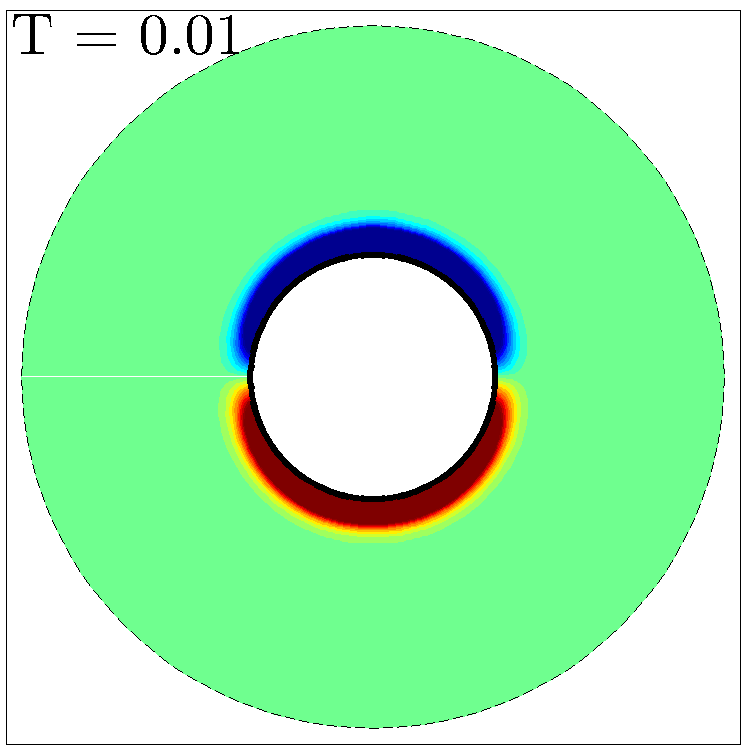
\includegraphics[width=6.5cm]{./Figures/vorticity_T0_01.eps} & 
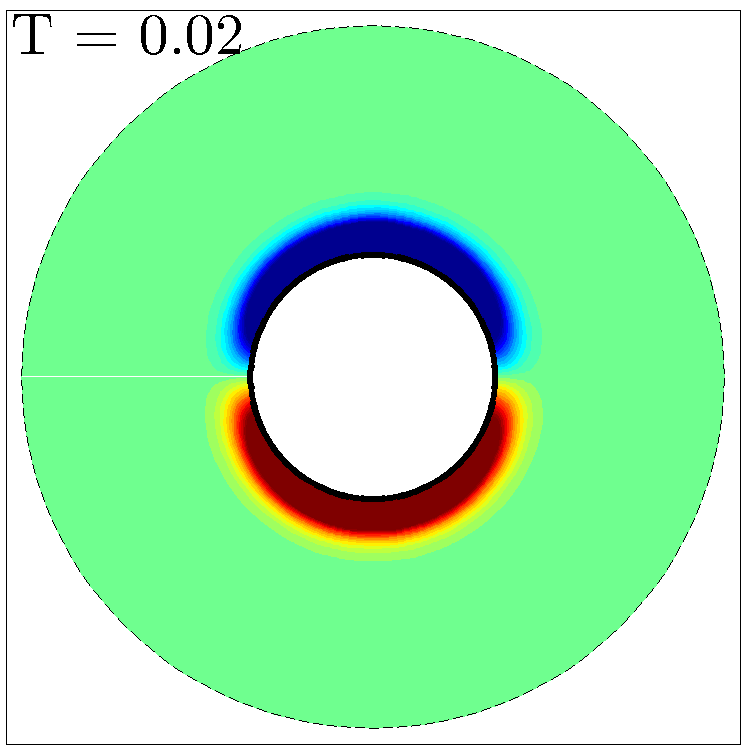
\includegraphics[width=6.5cm]{./Figures/vorticity_T0_02.eps}  \\
\includegraphics[width=6.5cm]{./Figures/vorticity_T0_03.eps} & 
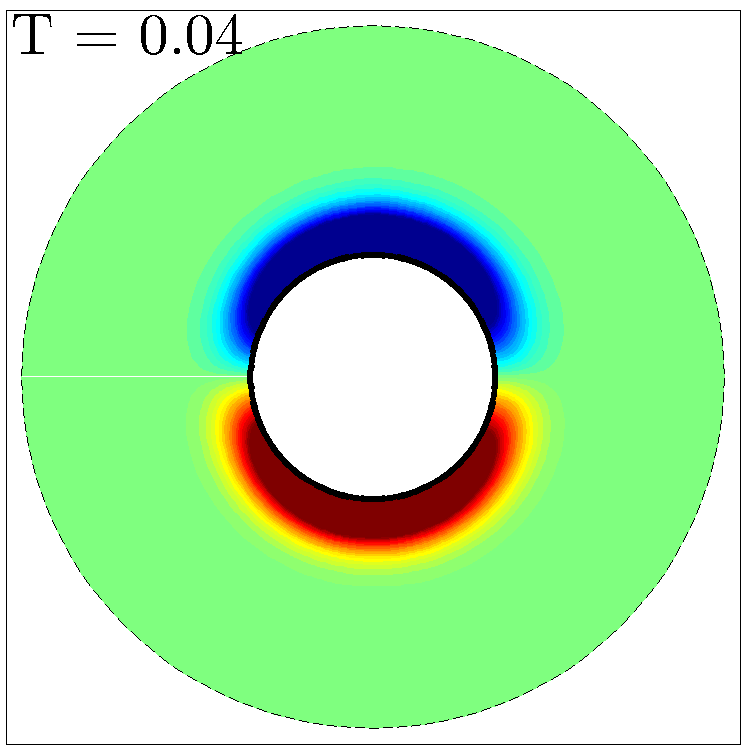
\includegraphics[width=6.5cm]{./Figures/vorticity_T0_04.eps} 
\end{tabular}
\end{center}
\caption[Initial vorticity profile inside boundary layer]{Initial vorticity development inside boundary layer (boundary layer thickness magnified for visualization)}
\label{fig:initialvorticity}
\end{figure}


\begin{figure}
\begin{center}
\begin{tabular}[t]{cc}
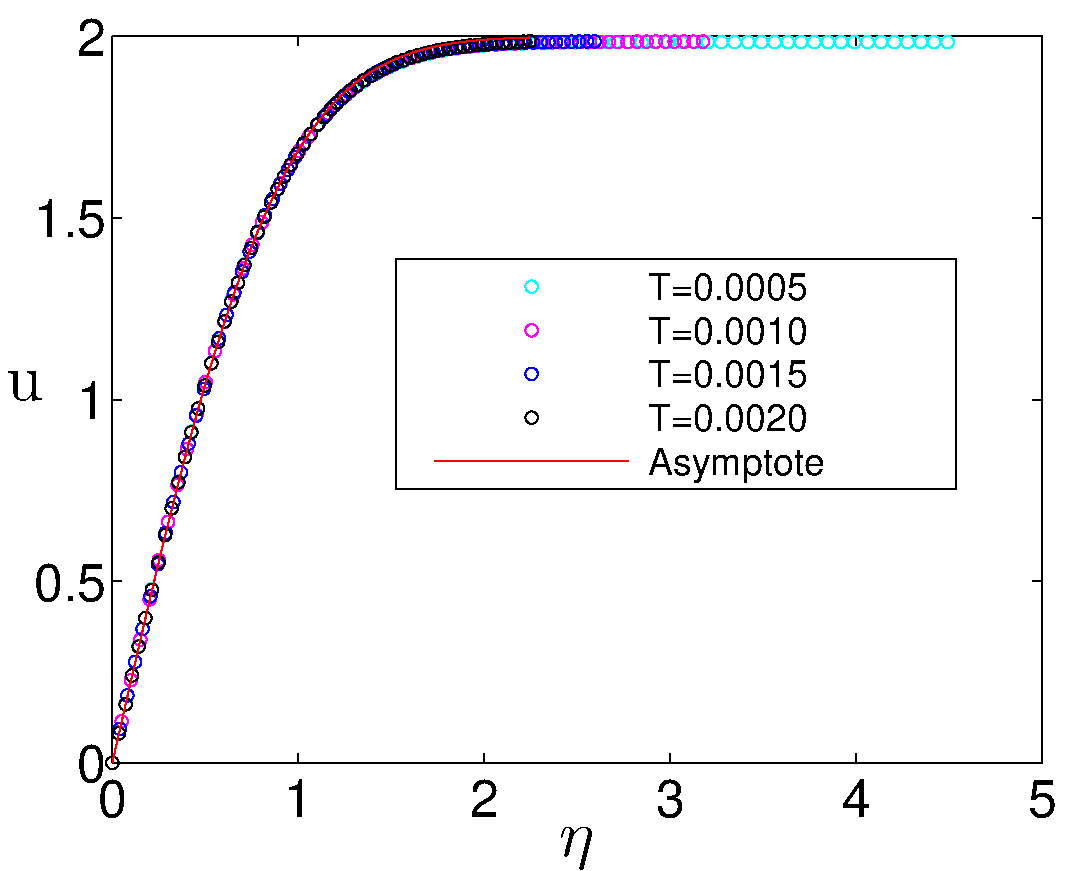
\includegraphics[width=6.5cm]{./Figures/u_asymptotic.eps} &
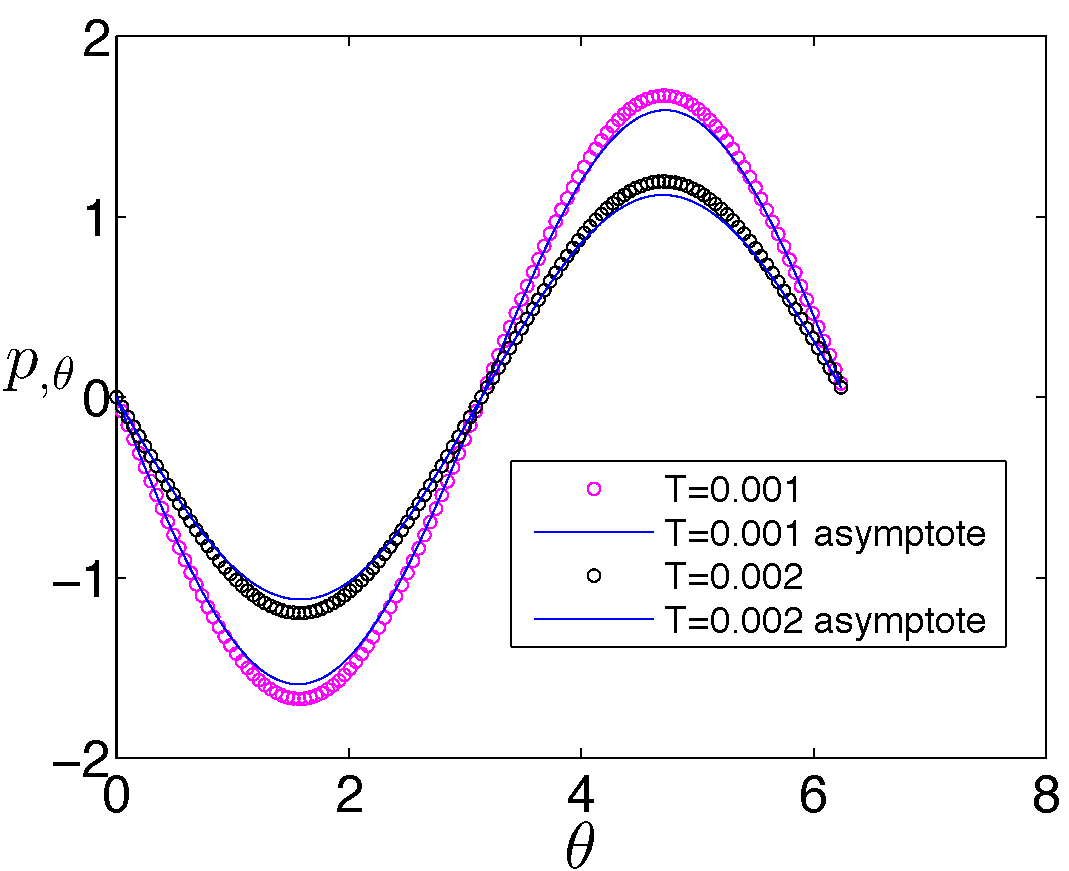
\includegraphics[width=6.5cm]{./Figures/p_asymptotic.eps} \\
(a) & (b) \\
\multicolumn{2}{c}{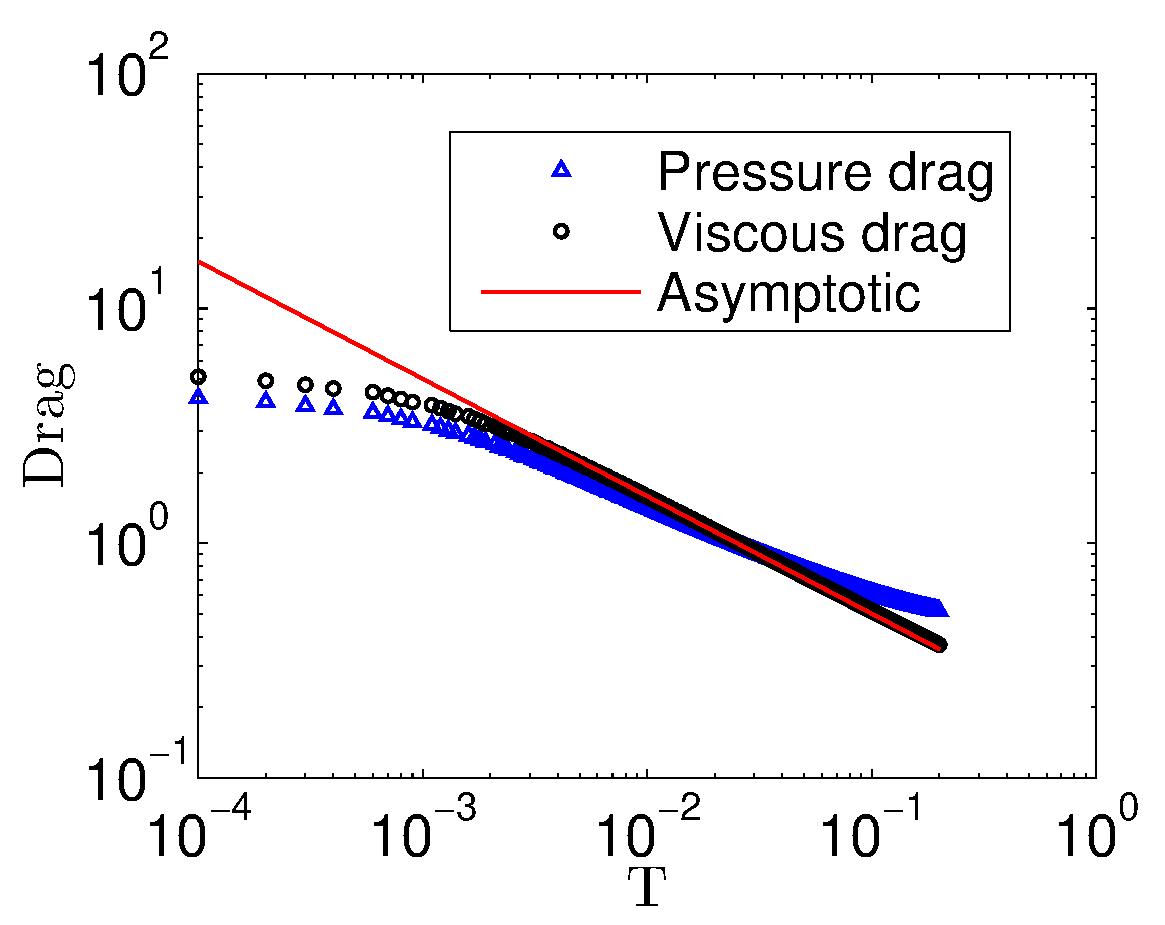
\includegraphics[width=10cm]{./Figures/InitialDrag.eps}} \\
\multicolumn{2}{c}{(c)}
\end{tabular}
\end{center}
 \caption[Initial flow properties compared with asymptotic solutions]{Initial flow properties compared with asymptotic solutions. (a) shows that tangential velocity profiles at $\theta = \pi/2$ at different times collapse to the asymptotic solution; (b) shows the perturbation of pressure to inviscid case; (c) shows the drag coefficients compared with asymptotic solution.}
 \label{fig:initialdrag}
\end{figure}


\begin{figure}
 \begin{center}
 \begin{tabular}{cc}
 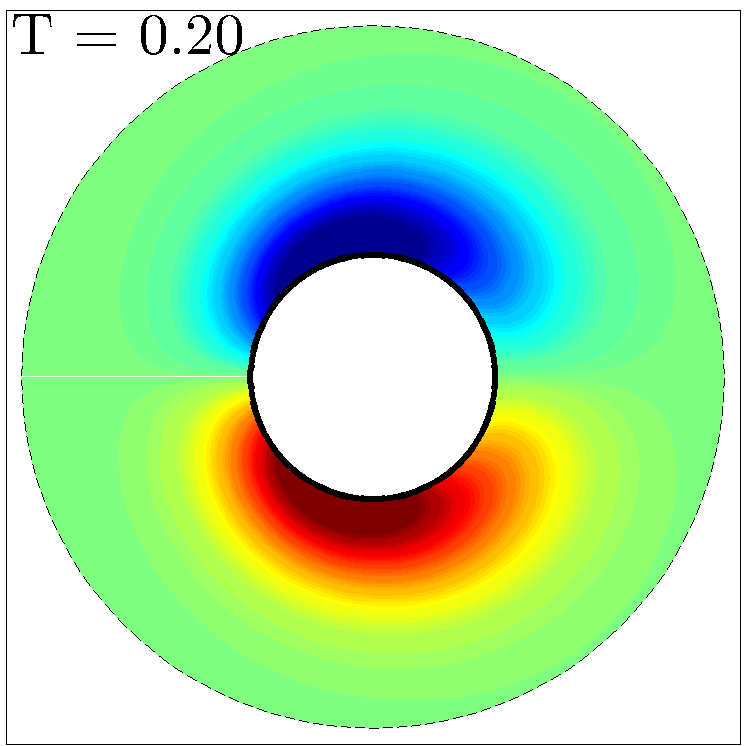
\includegraphics[width=5cm]{./Figures/vorticity_T0_20.eps} &
 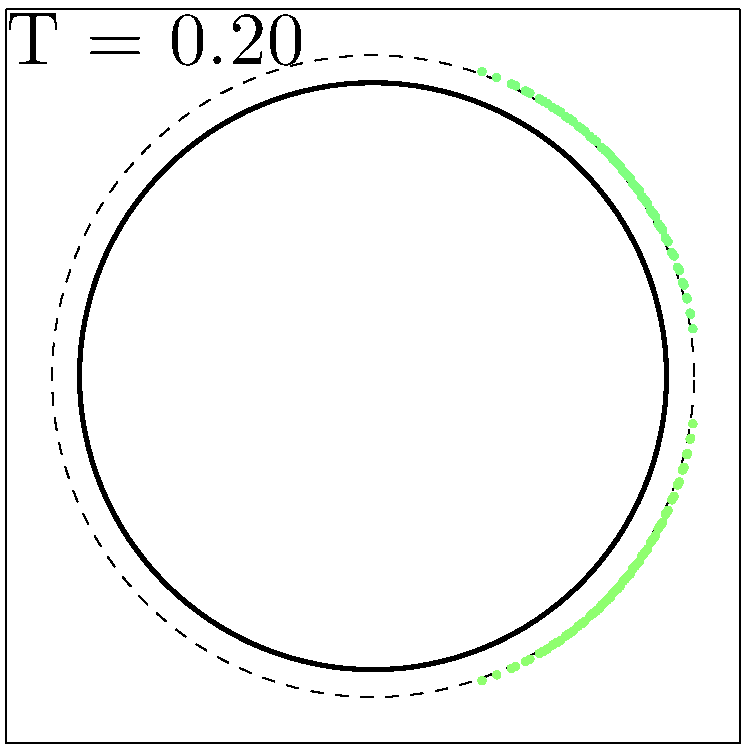
\includegraphics[width=5cm]{./Figures/vortices_T0_20.eps}  \\
 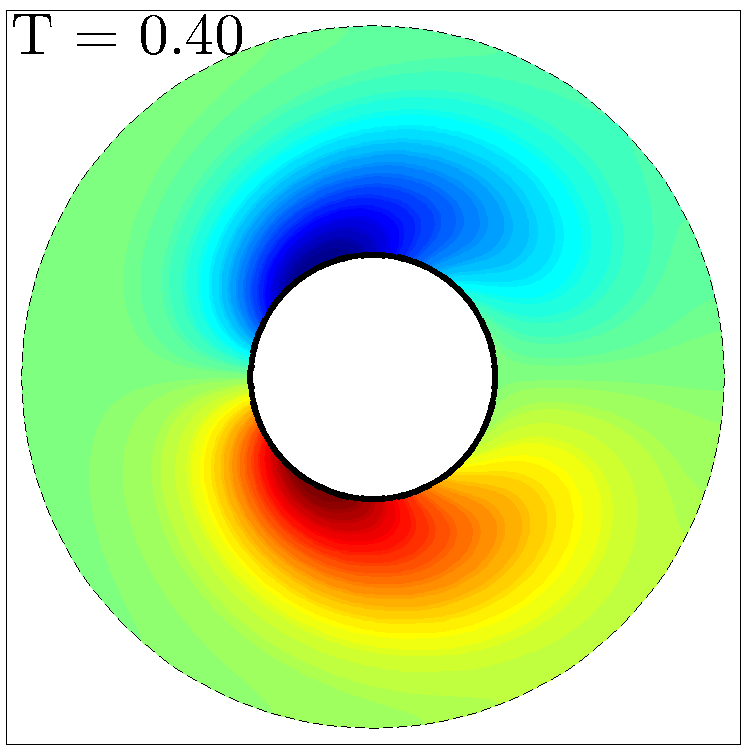
\includegraphics[width=5cm]{./Figures/vorticity_T0_40.eps} &
 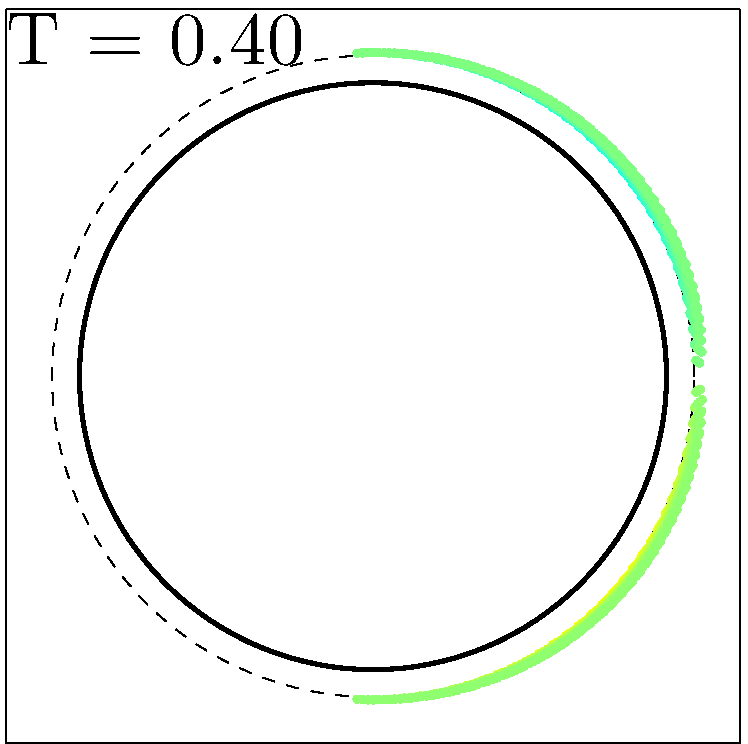
\includegraphics[width=5cm]{./Figures/vortices_T0_40.eps}  \\
 \includegraphics[width=5cm]{./Figures/vorticity_T0_60.eps} &
 \includegraphics[width=5cm]{./Figures/vortices_T0_60.eps}  \\
 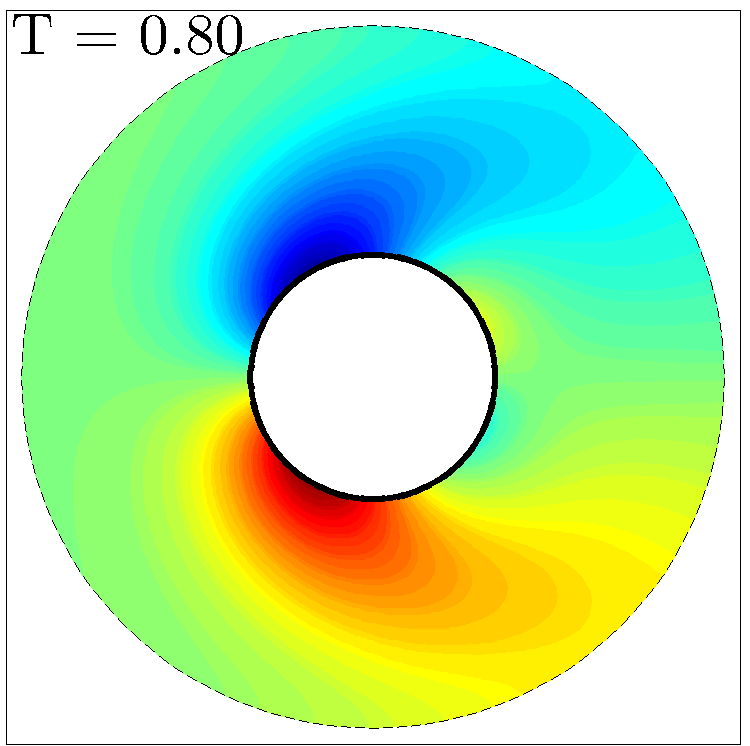
\includegraphics[width=5cm]{./Figures/vorticity_T0_80.eps} &
 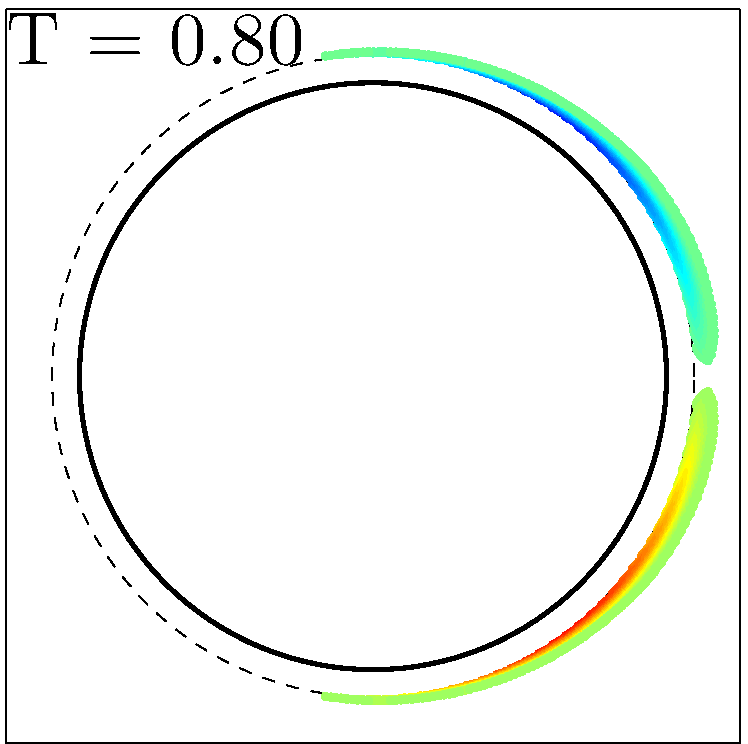
\includegraphics[width=5cm]{./Figures/vortices_T0_80.eps}  \\
 (a) & (b)
\end{tabular}
\end{center}
 \caption[Flow separates]{The flow separates (a) as the vorticity gets diffused and convected away from the body. When significant vorticity reaches the edge of boundary layer, certain amount of point vortices are shed into the outer region (b). }
 \label{fig:separation}
\end{figure}


\begin{figure}
 \begin{center}
 \includegraphics[width=10cm]{./Figures/separation_angle.eps}
 \end{center}
 \caption[Evolution of separation angle]{The time progression of separation angle compared with the direct numerical simulation result by KL.}
 \label{fig:separation_angle}
\end{figure}


\begin{figure}
 \begin{center}
 \begin{tabular}{cc}
 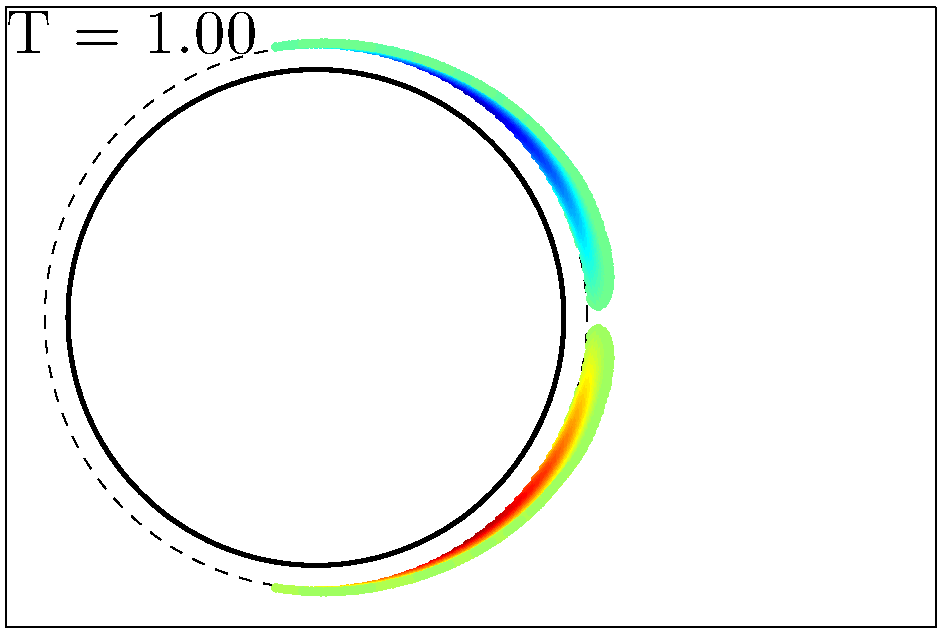
\includegraphics[width=6cm]{./Figures/vortices_T1_00.eps}  &
 \includegraphics[width=6cm]{./Figures/KOU_Re1000_T1.png}  \\
 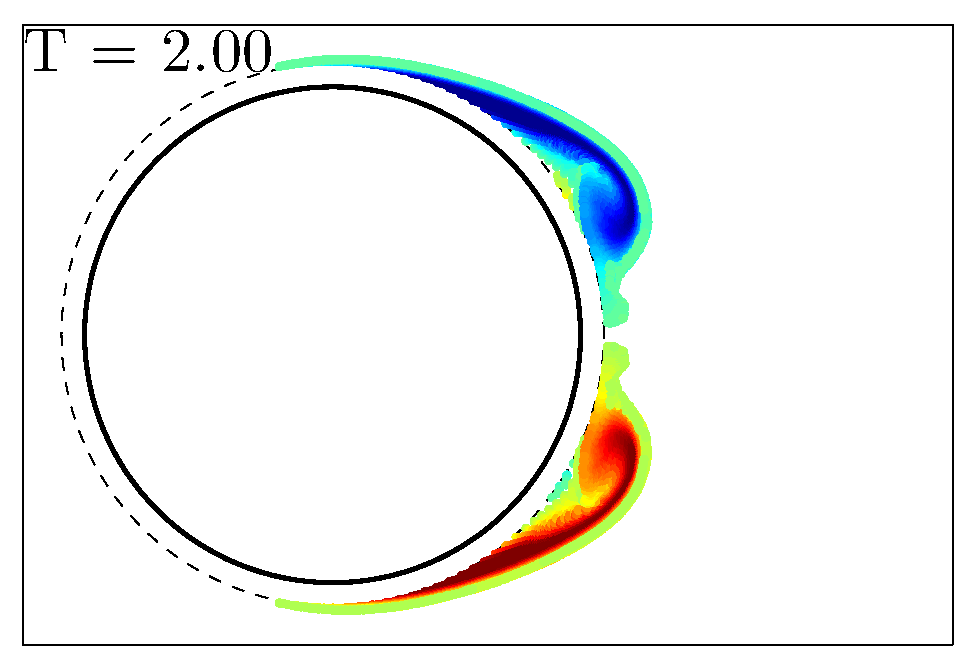
\includegraphics[width=6cm]{./Figures/vortices_T2_00.eps}  &
 \includegraphics[width=6cm]{./Figures/KOU_Re1000_T2.png}  \\
 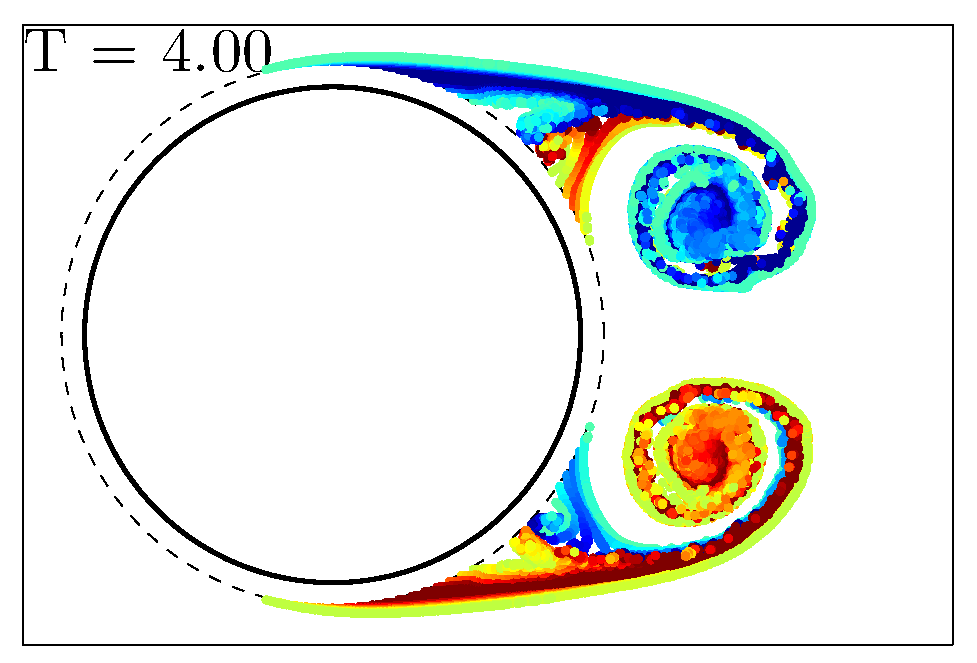
\includegraphics[width=6cm]{./Figures/vortices_T4_00.eps}  &
 \includegraphics[width=6cm]{./Figures/KOU_Re1000_T4.png}  \\
 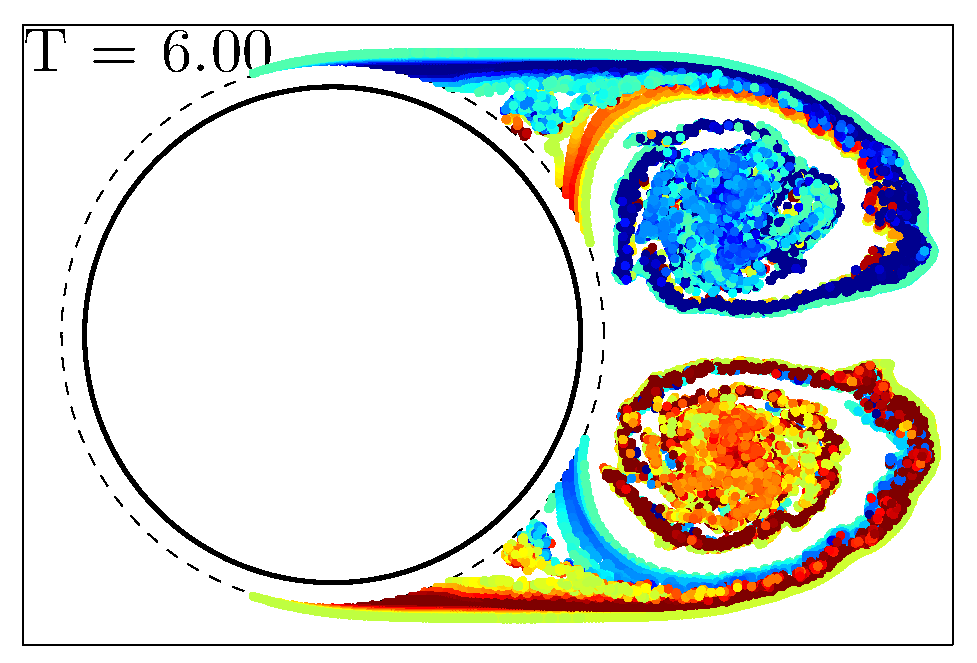
\includegraphics[width=6cm]{./Figures/vortices_T6_00.eps}  &
 \includegraphics[width=6cm]{./Figures/KOU_Re1000_T6.png}  \\
 (a) & (b) \\
 \end{tabular}
\end{center}
 \caption[Vortex shedding pattern in the wake]{The progression of vortex shedding pattern (a) with comparison to direct numerical simulation result by vortex methods (b). }
 \label{fig:wake}
\end{figure}


\begin{figure}
\begin{center}
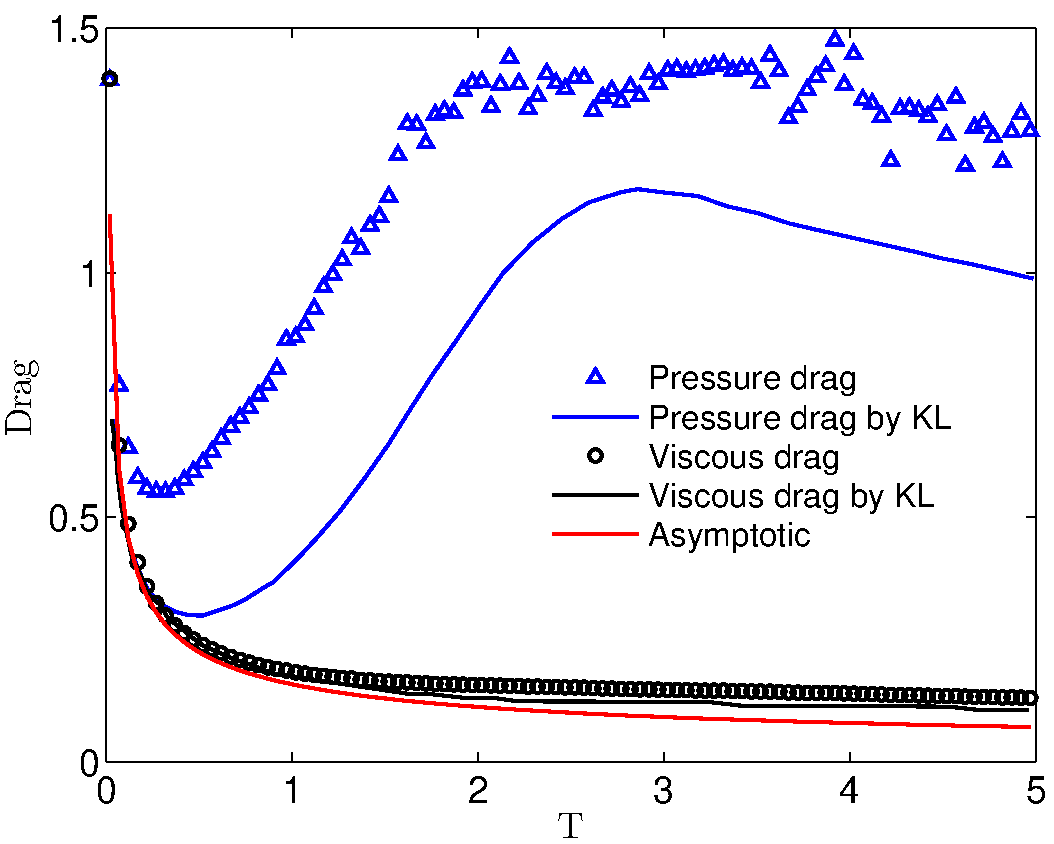
\includegraphics[width=10cm]{./Figures/Drag.eps}
\end{center}
\caption[Drag coefficient]{The drag coefficient compared with direct numerical simulation results and small-time asymptotic.}
\label{fig:Drag}
\end{figure}


\begin{figure}
\begin{center}
\includegraphics[width=10cm]{./Figures/Circulation.eps}
\end{center}
\caption[Total circulation in the upper-half plane]{Total circulation in the upper-half plane calculated with different boundary layer thickness $c/\sqrt{Re}$, compared with CFD result.}
\label{fig:Circulation}
\end{figure}

